% Использован шаблон:
% https://www.writelatex.com/coursera/latex/1.1
% http://coursera.org/course/latex


\documentclass[a4paper,12pt]{article}

\usepackage{cmap}
\usepackage[T2A]{fontenc}
\usepackage[utf8]{inputenc}
\usepackage[english,russian]{babel}
\usepackage{fancyhdr}
\usepackage{minted}
\usepackage{hyperref}
\usepackage{amsmath}
\usepackage{graphicx}
\usepackage{xcolor}

\hypersetup{
  pdfborderstyle={/S/U/W 1}
}

\graphicspath{{./images/}}

\pagestyle{fancy}
\fancyhf{}
\lhead{Антон Завьялов, ПИ-72}
\rhead{\textbf{Лабораторная №4. Вариант 7}}
\cfoot{\thepage}

\makeatletter
\def\@seccntformat#1{%
  \expandafter\ifx\csname c@#1\endcsname\c@section\else
  \csname the#1\endcsname\quad
  \fi}
\makeatother

\begin{document} % Конец преамбулы, начало текста.

\begin{center}
  \textbf{Лабораторная работа №4 по дисциплине\linebreak"Компьютерная графика"\linebreak\linebreakВыполнил студент группы ПИ-72 Завьялов А.А.}\\
\end{center}

\section{\normalsize{Задание}}
\begin{flushleft}
    Создать стационарное изображения  заданной трехмерной статичной сцены средствами OpenGL с использованием, возможно, стандартных геометрических примитивов.
    Обязательно наличие освещения, тени, текстуры и материала объектов, динамическая камера.
\end{flushleft}

\begin{flushleft}
  \textbf{Вариант 7.} Площадь города с памятником.
\end{flushleft}

\section{\normalsize{Исходный код}}
Исходный код программы также расположен в Git-репозитории по адресу: \url{https://github.com/andiogenes/cg/tree/master/scene}
\inputminted[breaklines]{c}{../main.c}

\section{\normalsize{Скриншоты, демонстрирующие работу программы}}
\begin{flushleft}
  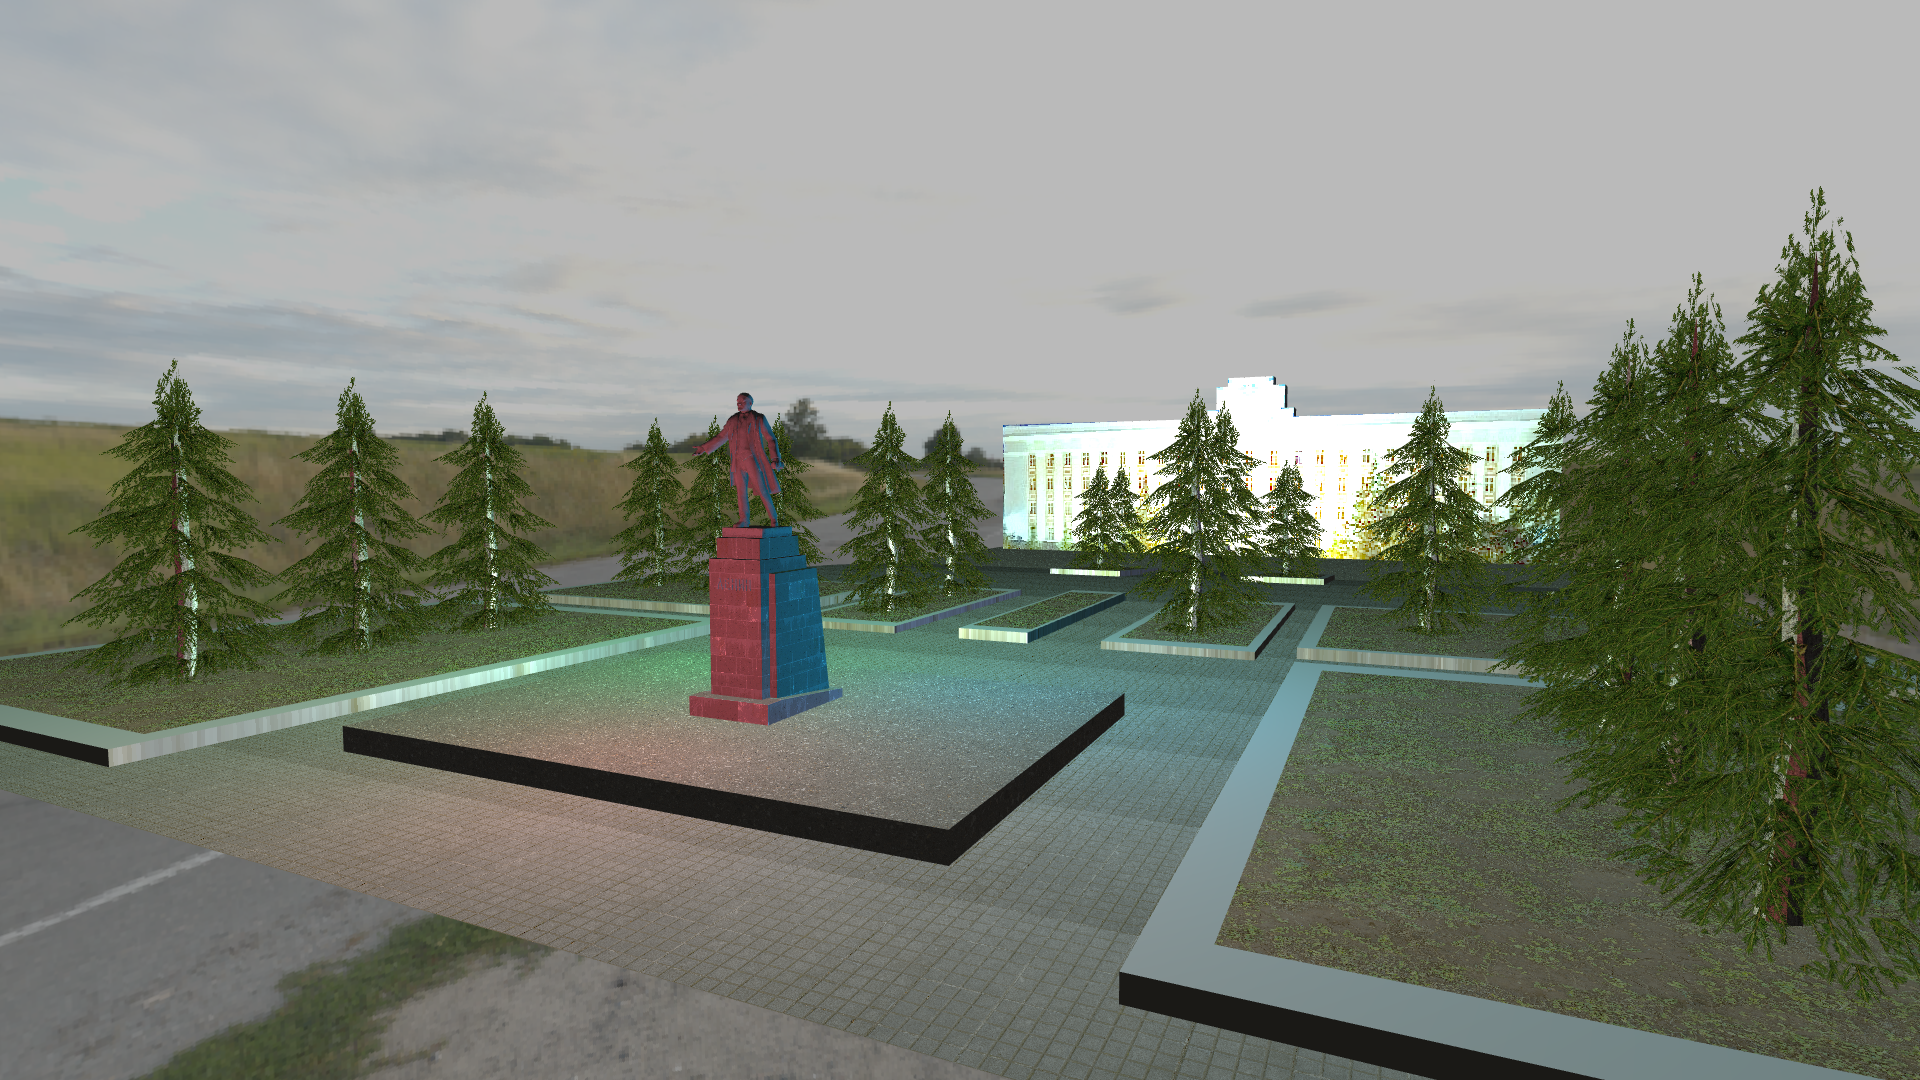
\includegraphics[scale=0.2]{screen_1.png}
  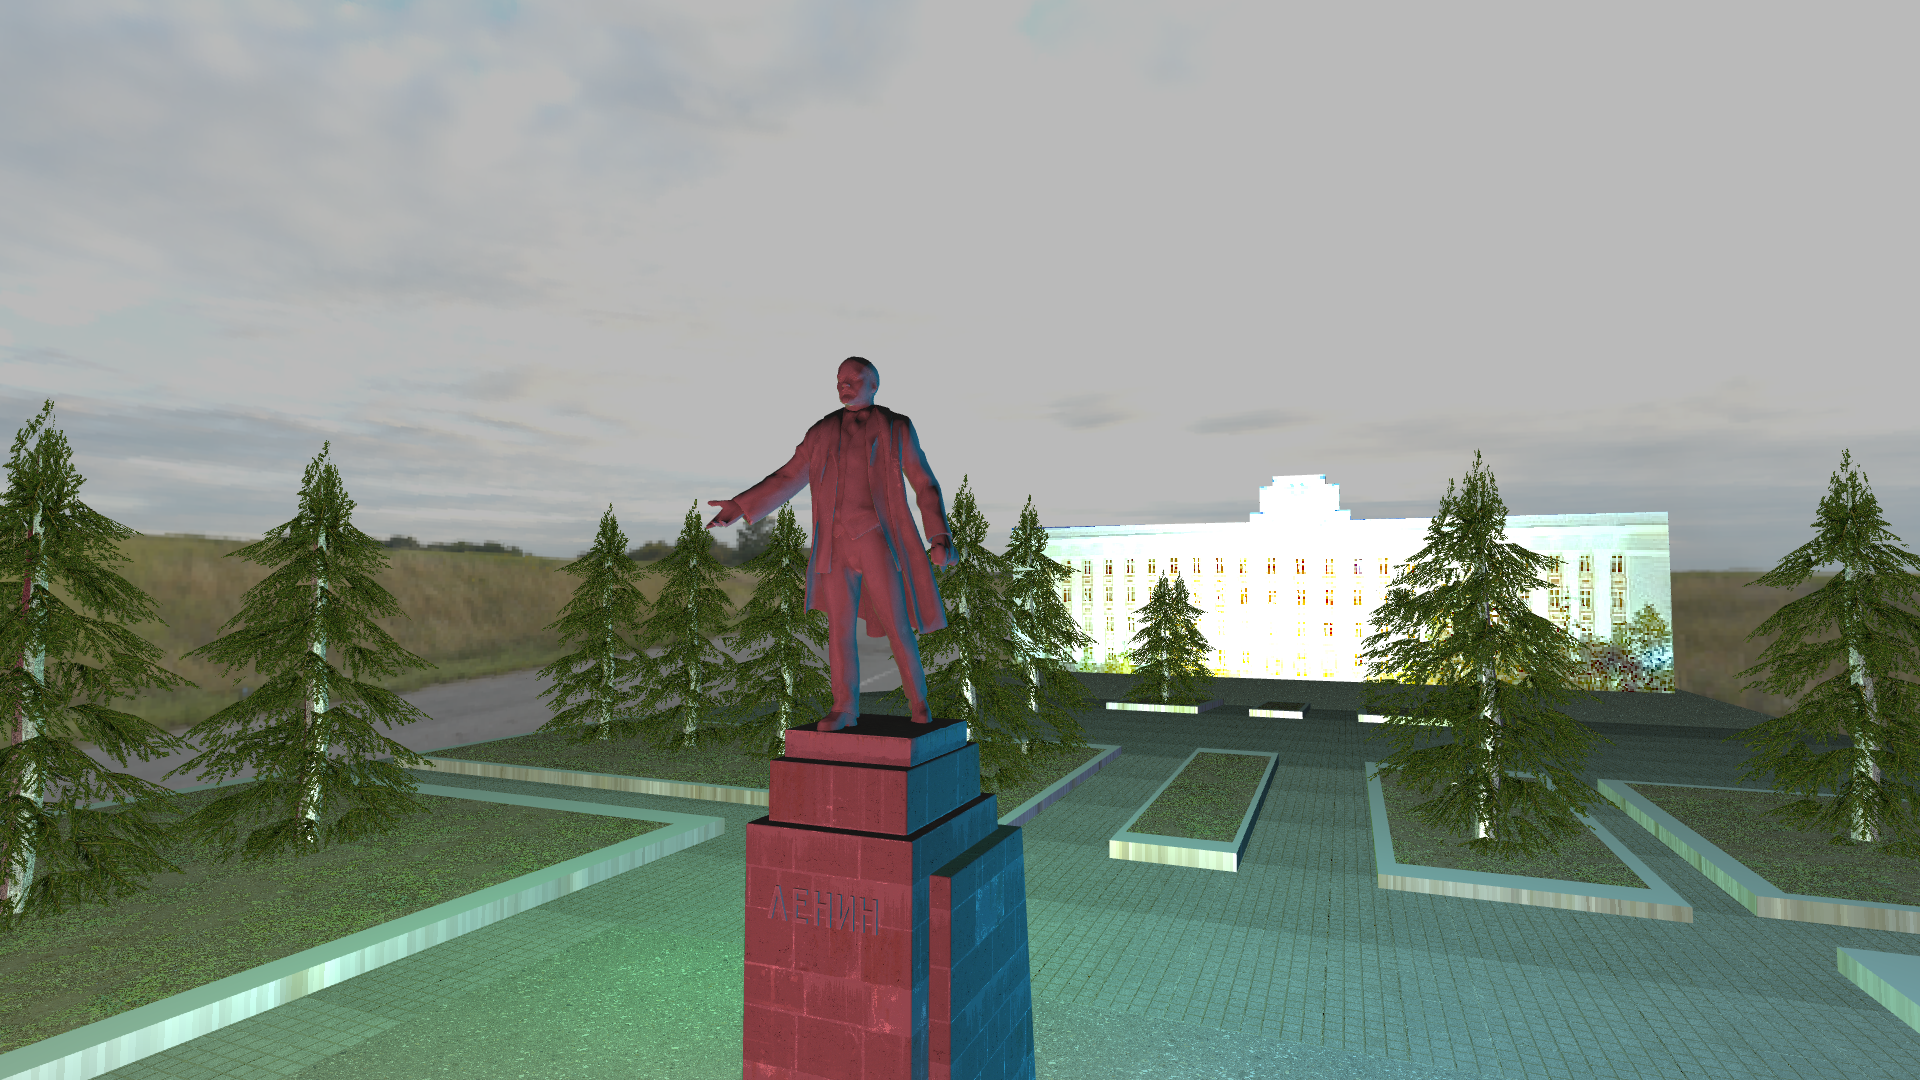
\includegraphics[scale=0.2]{screen_2.png}
  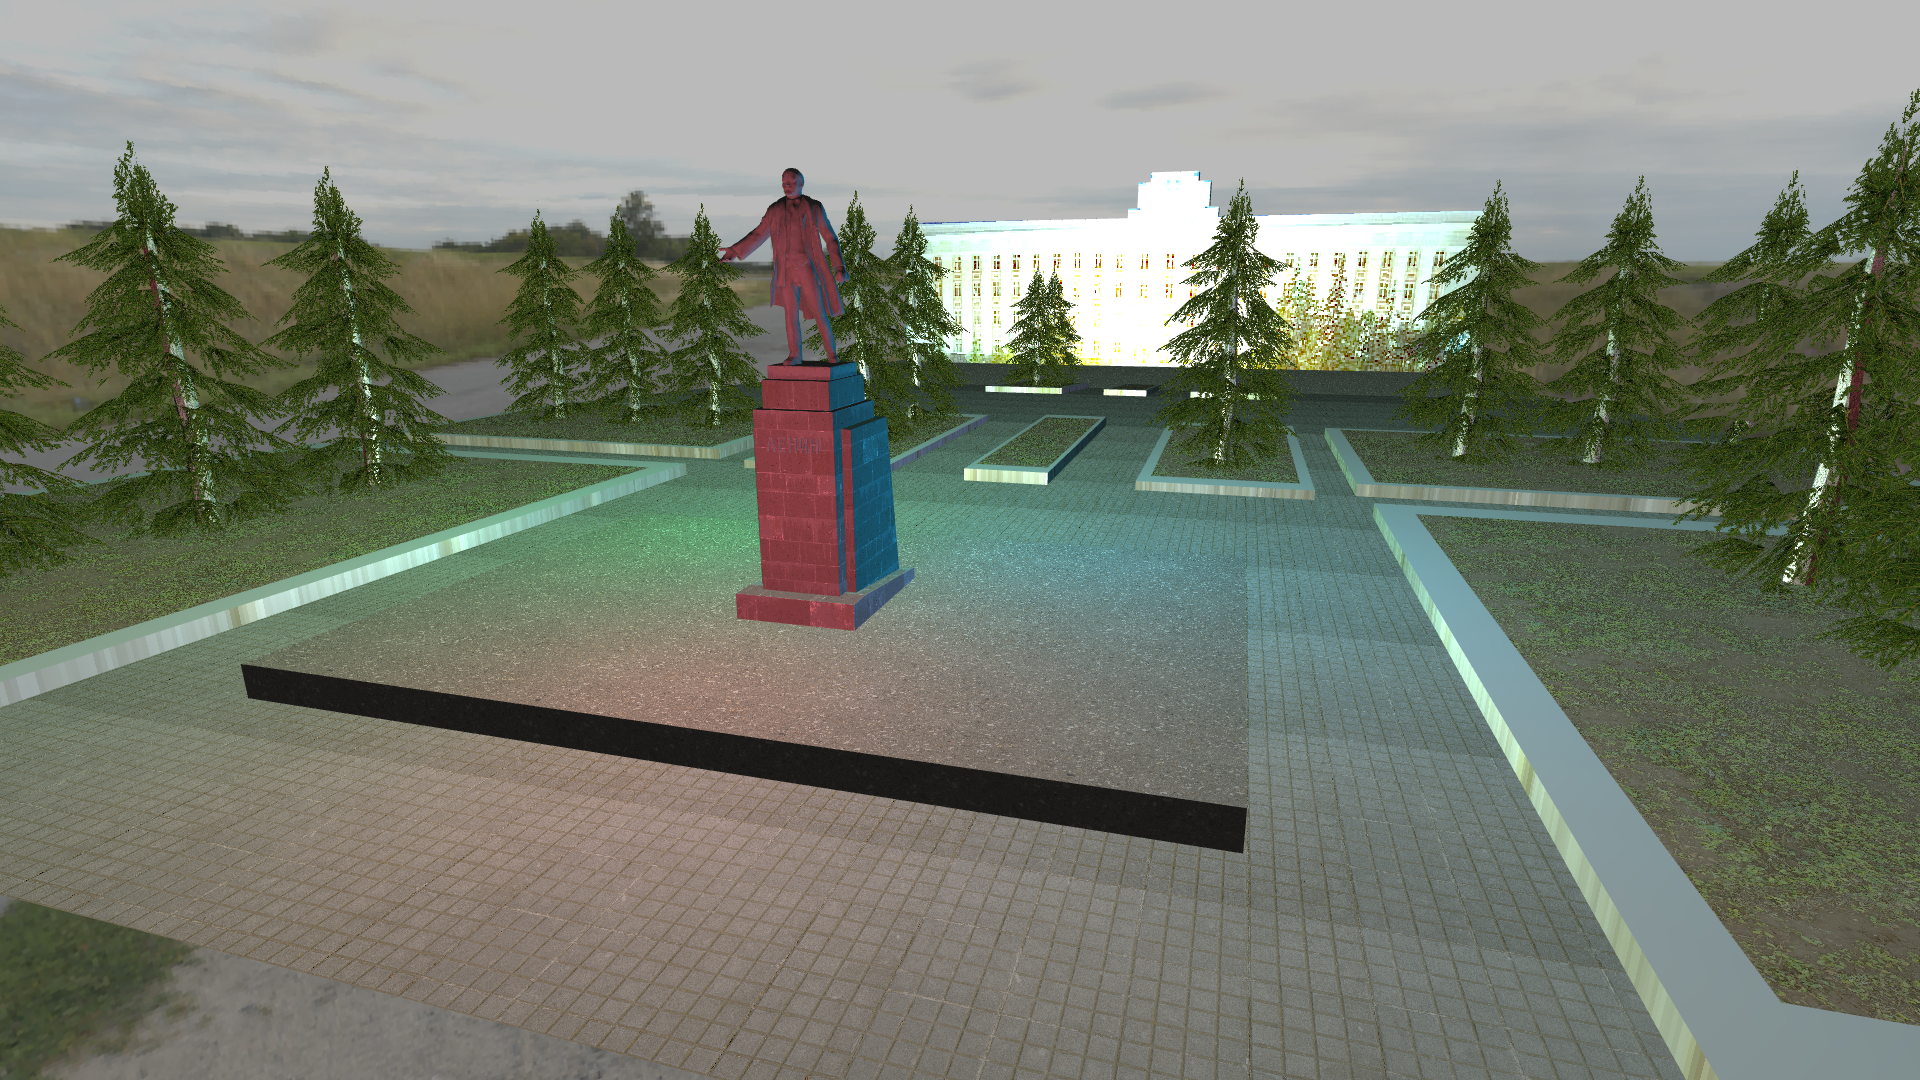
\includegraphics[scale=0.2]{screen_3.png}
  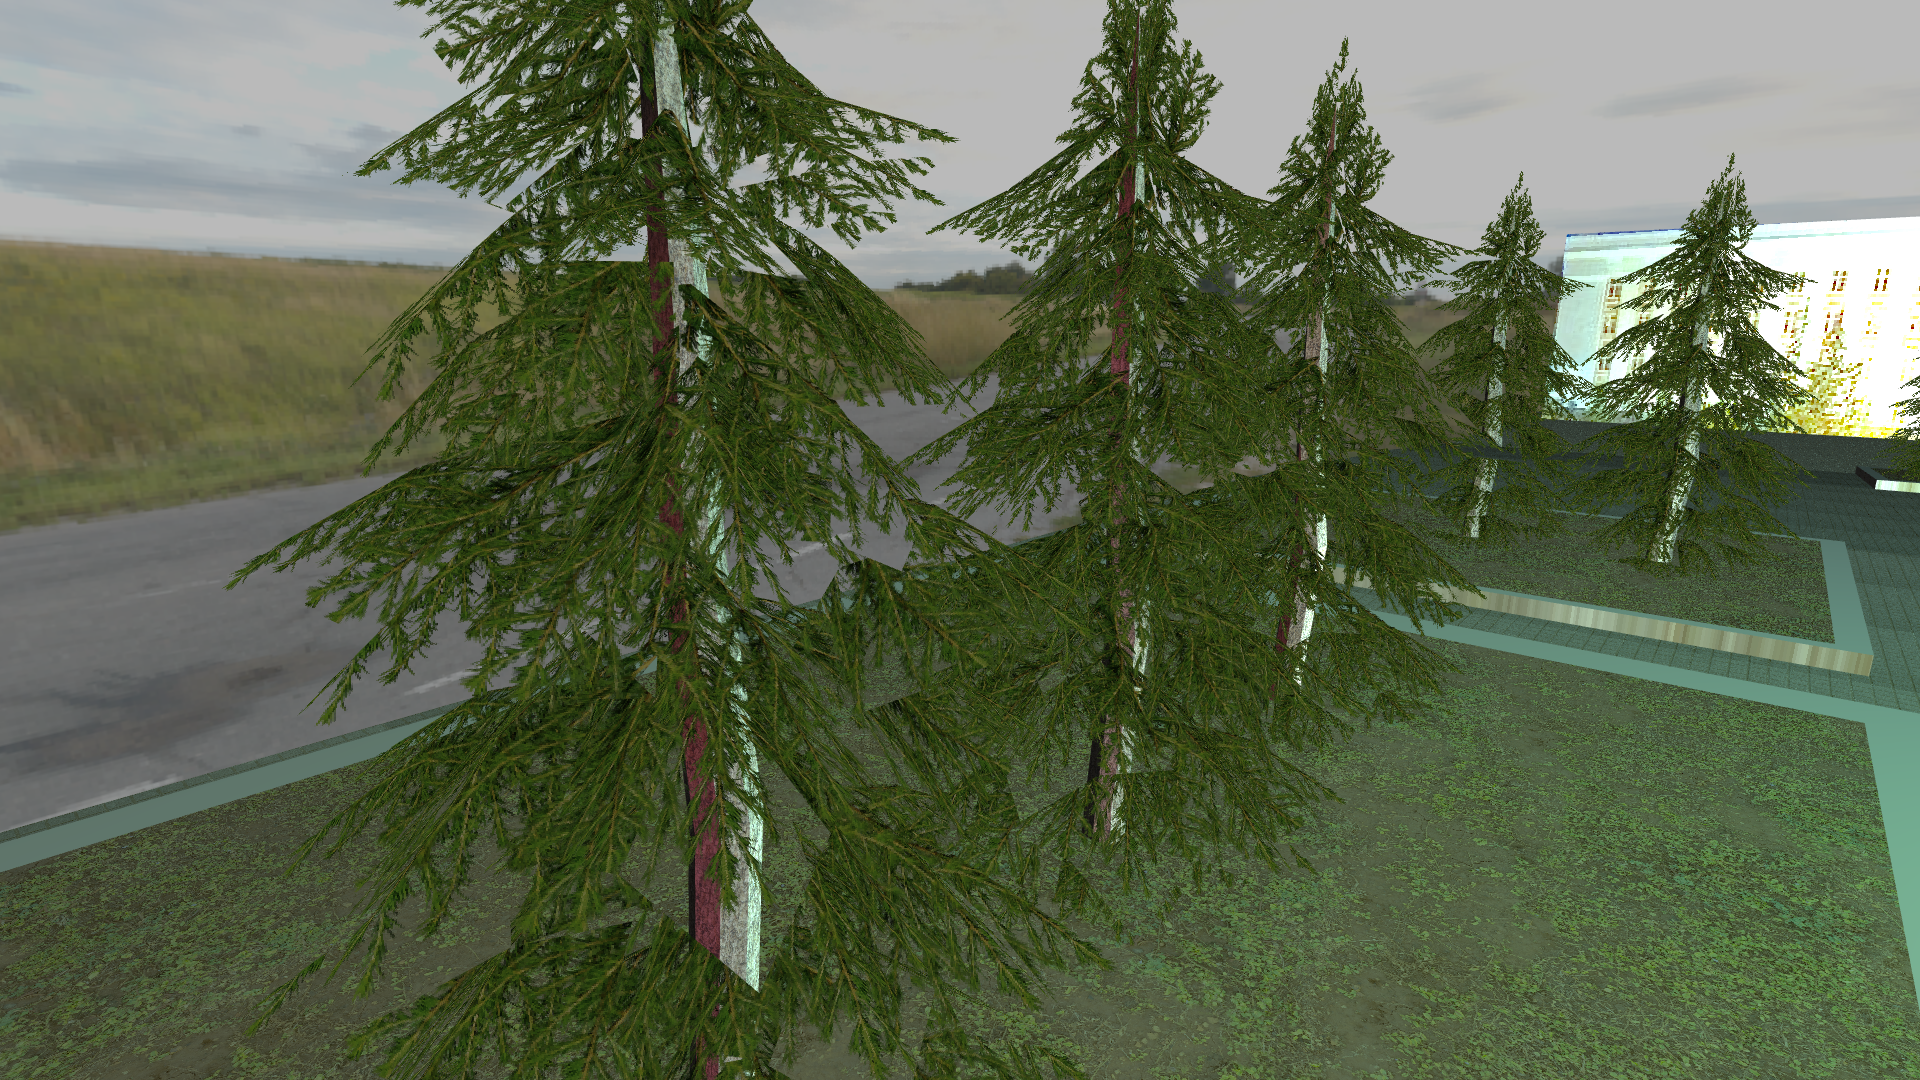
\includegraphics[scale=0.2]{screen_4.png}
  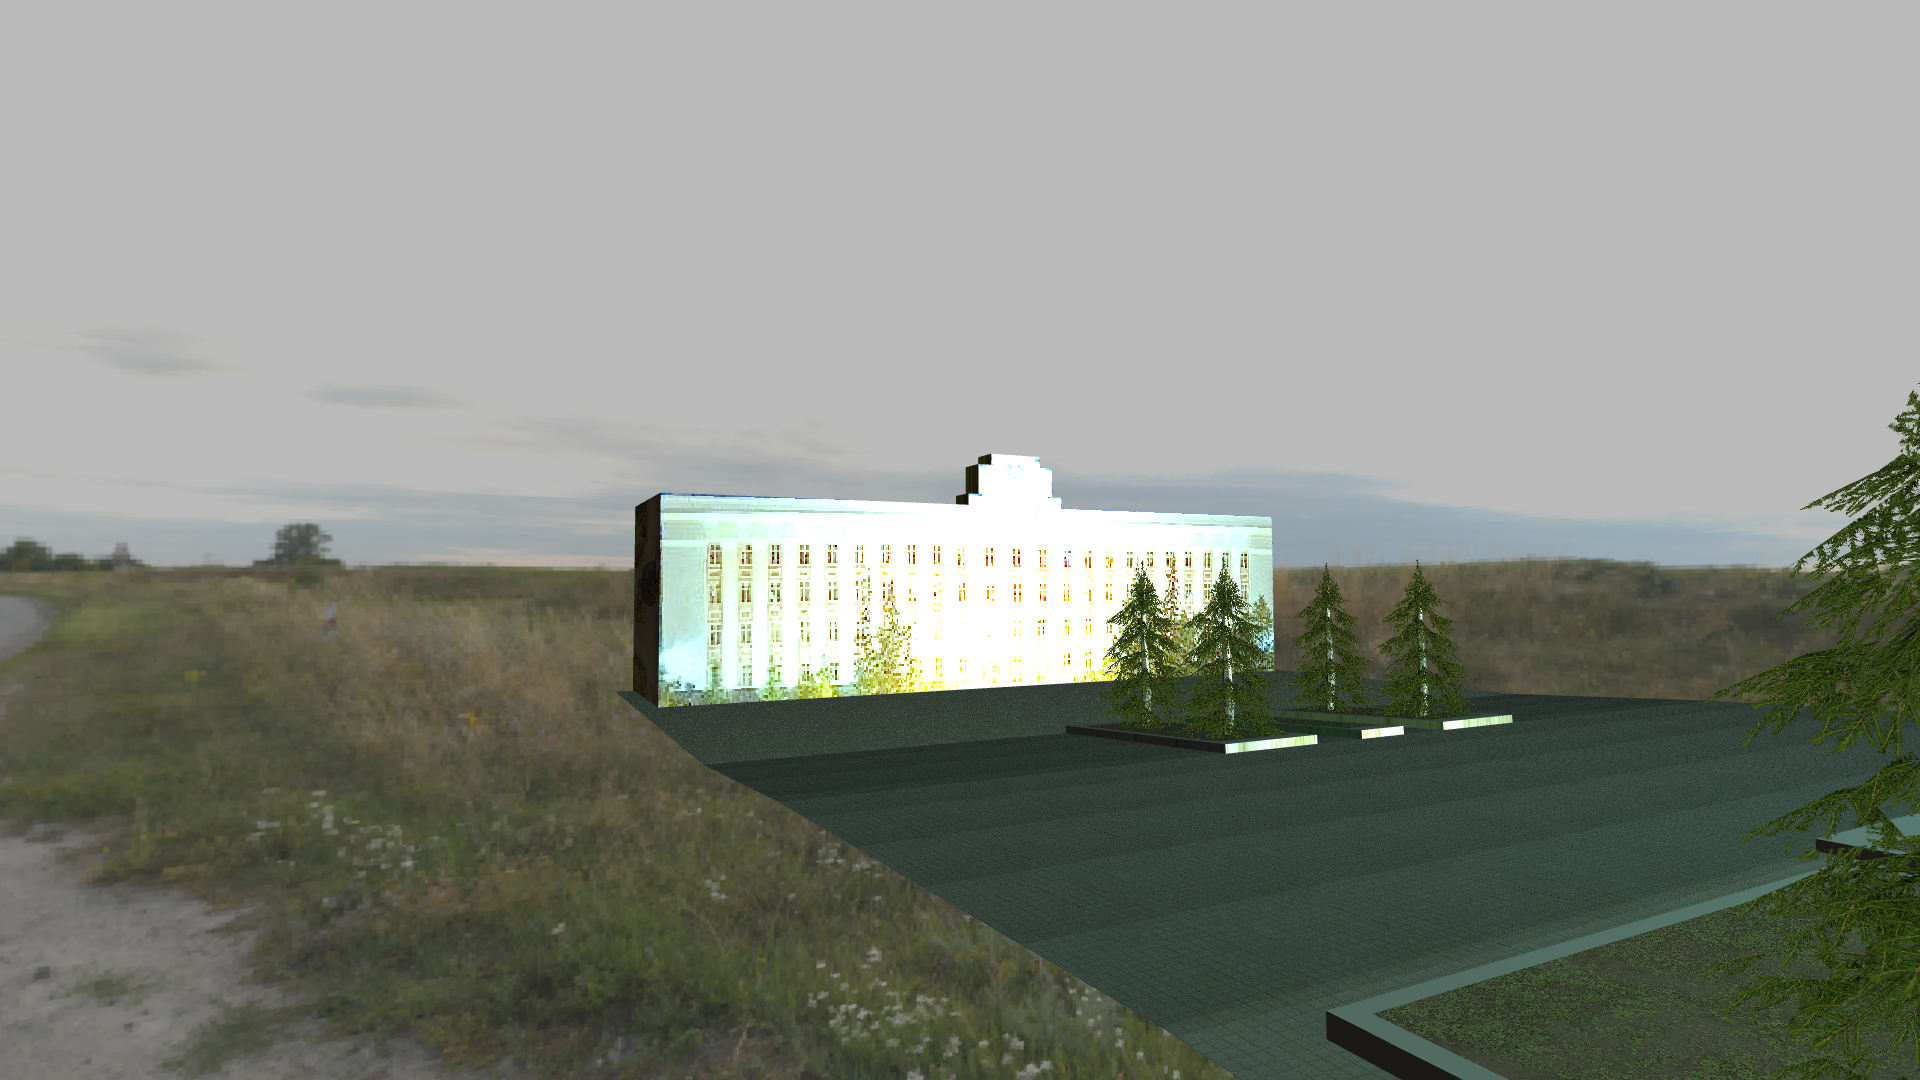
\includegraphics[scale=0.2]{screen_5.png}
\end{flushleft}
\end{document}

